\documentclass[11pt]{article}
\usepackage{amssymb}
\usepackage{amsmath}
\usepackage{amsthm}
\usepackage{fullpage}
\usepackage{hyperref}
\usepackage[h]{esvect}
\usepackage{graphicx}
\setlength{\parskip}{1ex}
\def\N {{\mathbb N}}
\def\Z {{\mathbb Z}}
\def\R {{\mathbb R}}
\newcommand{\Implies}{\mbox{ IMPLIES }}
\newcommand{\Or}{\mbox{ OR }}
\renewcommand{\And}{\mbox{ AND }}
\newcommand{\Not}{\mbox{NOT}}
\newcommand{\Iff}{\mbox{ IFF }}
\newcommand{\True}{\mbox{T}}
\newcommand{\False}{\mbox{F}}
\newcommand{\norm}[1]{\left| #1 \right|}
\usepackage{listings}
\usepackage{xcolor}
\usepackage{gensymb}

\definecolor{codegreen}{HTML}{237e02}
\definecolor{codegray}{rgb}{0.5,0.5,0.5}
\definecolor{codepurple}{HTML}{8F4673}
\definecolor{codebrown}{HTML}{ce9178}
\definecolor{codecyan}{HTML}{098658}
\lstdefinestyle{pythonstyle}{
    commentstyle=\color{codegreen},
    keywordstyle=\color{codepurple},
    numberstyle=\tiny\color{codegray},
    stringstyle=\color{codebrown},
    basicstyle=\ttfamily\small,
    breakatwhitespace=false,         
    breaklines=true,                 
    captionpos=b,                    
    keepspaces=true,                 
    numbers=none,                    
    numbersep=5pt,                  
    showspaces=false,                
    showstringspaces=false,
    showtabs=false,                  
    tabsize=2
}

\lstset{style=pythonstyle}

\begin{document}
\begin{center}

{\bf \Large \bf MATH209 Summer 2021 Problem Set 1 Part 2}\\
{\bf \large Kevin Gao}
\end{center}

\begin{enumerate}

    \item Question 4
    \begin{enumerate}
        \item
        Let $P_1$ and $P_2$ be two distinct points on the line of intersection of $x+2y-z=2$ and $3x+2y+2z=7$.
    
        Then the point must satisfy that
        $
        \begin{cases}
        x+2y-z=2 \\
        3x+2y+2z=7
        \end{cases}
        $
        
        Take $P_1 = (1,1,1)$ and $P_2=(-5,6,5)$. To define a line, we need a point and a direction vector. Let the direction vector $\vv{d}$ be the vector going from $P_1$ to $P_2$, that is $\vv d = (-6,5,4)$. Hence, that line is $\ell:\, (1,1,1) + (-6,5,4)t$. whose parametric form is
        $$
        \begin{cases}
        x = -6t+1 \\
        y = 5t+1 \\
        z = 4t+1
        \end{cases}
        $$
        Since $\ell_1$ has the direction vector $\vv d = (-6,5,4)$ while the direction vector for the other line is $\vv d_1 = (6,-5,-4)$. Let $k = -1$. Then, there exists a $k \in \R$ such that $\vv d = k\vv d_1$. It follows that the direction vectors are parallel.
        
        Therefore, the two lines are parallel.
        
        \item
        Let $\pi_3$ be the plane defined by the two lines.
    
        Let $P_3$ be a point on the line $x=1+6t,\, y=3-5t,\, z=2-4t$. Take $t=1$. Then, $P_3=(7,-2,-2)$.
        
        Define $\vv v$ be the vector going from $P_1$ to $P_3$. So, $\vv v = (6,-3,-3)$. Since $\pi_3$ is the plane defined by the two lines, $P_1,P_2,P_3$ are all points on the plane, and $\vv d$ and $\vv v$ are on the plane.
        
        Take the cross product $N=\vv d \times \vv v = (-3,6,-12)$. $N$ is perpendicular to both vectors, making $N$ a normal of the plane.
        
        In addition, since the plane passes through $P_1=(1,1,1)$, we can define the plane as follows:
        $$
        \pi:\, -3(x-1)+6(y-1)-12(z-1)=0
        $$
    \end{enumerate}

    \item Question 7
    
    Let $\ell_1$ be the line $x=3t,\,y=1+t,\,z=2-t$. 
    
    Let $P_2$ and $P_3$ be two distinct points on $\ell_t$. Take $t=1,2$, which gives $P_2=(3,2,1),\, P_3=(6,3,0)$. These two points, along with the given point $P_1=(1,2,3)$, allow us the define a plane.
    
    Let $\pi$ be such plane. Define $\vv v$ be the vector from $P_2$ to $P_3$, and $\vv u$ be the vector from $P_1$ to $P_2$. Then, $\vv v = (3,1,-1)$ and $\vv u = (2,0,-2)$.
    
    Taking the cross product of $N = \vv v \times \vv u = (-2,4,-2)$. This is a normal of the plane. Since the plane passes through the point $P_1=(1,2,3)$, the plane can be defined as
    
    $$
    \pi:\, -2(x-1)+4(y-2)-2(z-3)=0
    $$
    
    \item Question 14
    
    To define a line, we need two points. Let $P_1,P_2$ be two distinct points on the intersection of the two planes. Then, the coordinates must satisfy 
    $
    \begin{cases}
    3x-2y+z=1 \\
    2x+y-3z=1
    \end{cases}
    $
    Take $P_1=(4,8,5)$ and $P_3=(9,19,12)$. Then, we can define the direction vector $\vv d = (5,11,7)$.
    
    From the direction vector and $P_1$, we can define the line:
    $$
    \ell:\, (4,8,5)+(5,11,7)t
    $$
    which can be written in parametric form as $x=4+5t,\,y=8+11t,\,z=5+7t$.
    
    The angle between the planes is equal to the angle between their normals, which can be calculated using dot product.
    $$
    \sin\theta = \frac{(3,-2,1)\cdot (2,1,-3)}{\sqrt{14} \cdot \sqrt{14}} = 1
    $$
    It follows that $\theta = \arcsin(1) = 90\degree$

    \newpage
    
    \item Question 15
    
    Let $\pi$ be a plane passing through $(1,3,-2)$. Then,
    $$
    \pi:\, a(x-1)+b(y-3)+c(z-2) = 0
    $$
    Let $\ell$ be the line that is the intersection of $x-y+z=1$ and $x+y-z=1$.
    
    Suppose that $x=1$, we can have two points $(1,0,0)$ and $(1,2,2)$ that is on the line intersecting $x-y+z=1$ and $x+y-z=1$.
    
    From the two points, we can calculate the direction vector $\vv{d} = (0,2,2)$.
    
    Let $\vv{v}$ be the vector going from $(1,0,0)$ to $(1,3,-2)$. Then, $\vv{v}=(0,3,-2)$. Since $\pi$ contains the point $(1,3,-2)$ and the line with direction vector $\vv{d}$, the normal of that plane must be perpendicular to both $\vv{d}$ and $\vv{v}$. We can find the normal by taking the cross product:
    $$
    N = \vv{d} \times \vv{v} = (2,0,0)
    $$
    from which we can define the plane as
    $$
    \pi:\, 2(x-1) = 0
    $$
    
    \begin{figure}[h!]
        \centering
        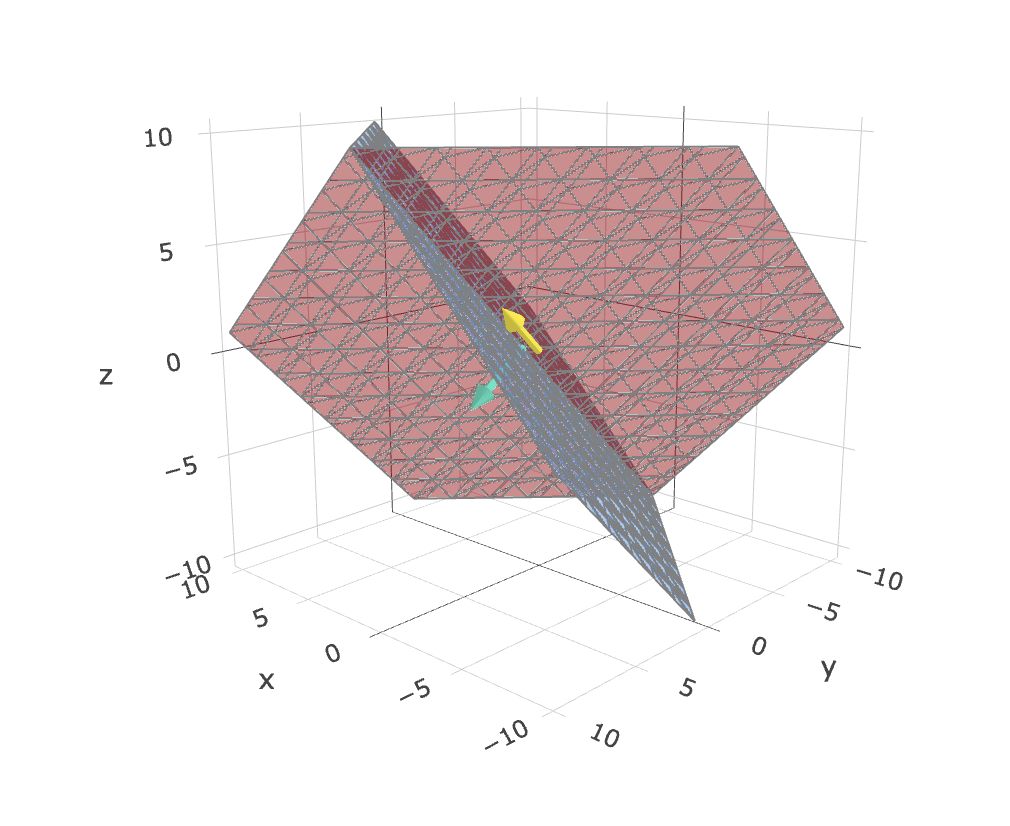
\includegraphics[width=0.5\linewidth]{figures/p2q15.png}
    \end{figure}
    
    \item Question 18
    
    Let $P$ be the point on the line that is the closest to $(0,1,3)$. Since $P$ is on the line, there exists some $t \in \R$ such that $P=(2t,6-2t,3+5t)$.
    
    Let $\vv v$ be the vector from $(0,1,3)$ to $P$. Then, $\vv v = (2t,5-2t,t)$. $\vv v$ is the vector connecting the shortest path between the point and the line. Let $\vv d = (2,-2,1)$ be the direction vector of the line.
    
    Since $P$ is the closest point to $(0,1,3)$ on the line. $\vv v$ must be orthogonal to the direction vector of that line. It follows that $\vv v \cdot \vv d = 0$
    
    \begin{align*}
        (2t,5-2t,t) \cdot (2,-2,1) &= 0 \\
        4t-10+4t+t &= 0 \\
        9t &= 10 \\
        t &= 10/9
    \end{align*}
    
    Substituting the value of $t$ back to the coordinate of $P$ gives us $P=(20/9,34/9,37/9)$. Then the distance between the point $(0,1,3)$ and the line is just the distance between the point and $P$.
    
    $$
    D=\sqrt{(\frac{20}{9}-0)^2 + (\frac{34}{9}-1)^2 + (\frac{37}{9}-3)^2} = \frac{5\sqrt{5}}{3}
    $$
    
    \item Question 22
    
    Define the following vectors:
    \begin{align*}
        \vv{QP}&= (2,0,-1)-(4,1,0) = (-2,-1,-1) \\ \vv{QR}&=(3,-1,1)-(4,1,0) = (-1,-2,1) \\ \vv{QS}&=(a,-2,2)-(4,1,0) = (a-4,-3,2)
    \end{align*}
    Then, the volume of the parallelepiped is given by the absolute value of triple product
    $$
    V=|\vv{QP} \cdot (\vv{QR}\times\vv{QS})|=-9-3a
    $$
    Its volume is zero when $a=3$.
    \item Question 25
    \begin{enumerate}
        \setcounter{enumii}{1}
        \item 
        Let
        $$
        \begin{cases}
        \frac{x-1}{2}=\frac{y}{3}=\frac{z-2}{-1} = t \\
        \frac{x+1}{1}=\frac{y-4}{1}=\frac{z-1}{3} = u
        \end{cases}
        $$
        from which we can convert the equation of the lines into vector form: $L_1:\, (1,0,2)+(2,3,-1)t$ and $L_2:\, (-1,4,1)+(1,1,3)u$.
        
        Since $(1,1,3)$ is not a scalar multiple of $(2,3,-1)$, the two lines are not parallel.
        
        To see if they intersect, consider this system of linear equations
        $$
        \begin{cases}
        2t+1=u-1 \\
        3t=u+4 \\
        -t+2=3u+1
        \end{cases}
        $$
        The system of linear equation is inconsistent and does not have a solution. So the lines do not intersect either.
        
        Hence the lines are skew.
        
        To find the distance between the lines, we first take a point on $L_1$. Let $P_1=(1,0,2)$ be that point. Since $L_1$ is skew to $L_2$, then the planes containing $L_1$ and $L_2$ are parallel. Then, the two planes share a same normal.
        $$
        N=(2,3,-1) \times (1,1,3) = (10,-7,-1)
        $$
        Then, the plane containing $L_1$ is $10(x-1)-7y-(z-2)$
        
        The distance from $L_1$ to $L_2$ can then be expressed as the distance between an arbitrary point on $L_2$ and the plane containing $L_1$.
        
        $$
        D = \frac{|ax_1+by_1+cz_1+d|}{\sqrt{a^2+b^2+c^2}} = \frac{10\cdot (-1) -7 \cdot 4 - 1 - 8}{\sqrt{10^2+7^2+1^2}} = \frac{47\sqrt{6}}{30}
        $$
        
        \item
        Let
        $$
        \begin{cases}
        \frac{x-2}{1}=\frac{y-6}{-1}=\frac{z+2}{3} = t \\
        \frac{x-1}{2}=\frac{y-3}{2}=\frac{z-2}{-1} = u
        \end{cases}
        $$
        from which we can convert the equation of the lines into vector form: $L_1:\, (2,6,-2)+(1,-1,3)t$ and $L_2:\, (1,3,2)+(2,2,-1)u$.
        
        Since $(2,2,-1)$ is not a scalar multiple of $(1,-1,3)$, the two lines are not parallel.
        
        To see if they intersect, consider this system of linear equations
        $$
        \begin{cases}
        t+2=2u+1 \\
        -t+6=2u+3 \\
        3t-2=-u+2
        \end{cases}
        $$
        The system of linear equation has a solution
        $
        \begin{cases}
        t = 1\\
        u = 1
        \end{cases}
        $
        Hence the lines intersect each other. The intersection point is $(3,5,1)$
    \end{enumerate}
\end{enumerate}

\end{document}